\newpage
\section{CSVL Vs CSVM fat jet b tagging}
In H(bb)Z analysis, We compare the csvl fat jet b tagging vs csvm on the limits. 
Fig.\ref{fig:HbbCSVMDijetMass} is showing the dijet mass spectrum with CSVL fat jet b tagging vs CSVM. 
And Fig.\ref{fig:HbbLimitsCompare} is showing the limits comparison between CSVL fat jet b tagging Vs CSVM. 
On the table, the limits from CSVL and CSVM are very close, so we show the limits in Table.\ref{table:HbbCSVM}. 


\begin{figure*}[h!tpb]
\begin{center}
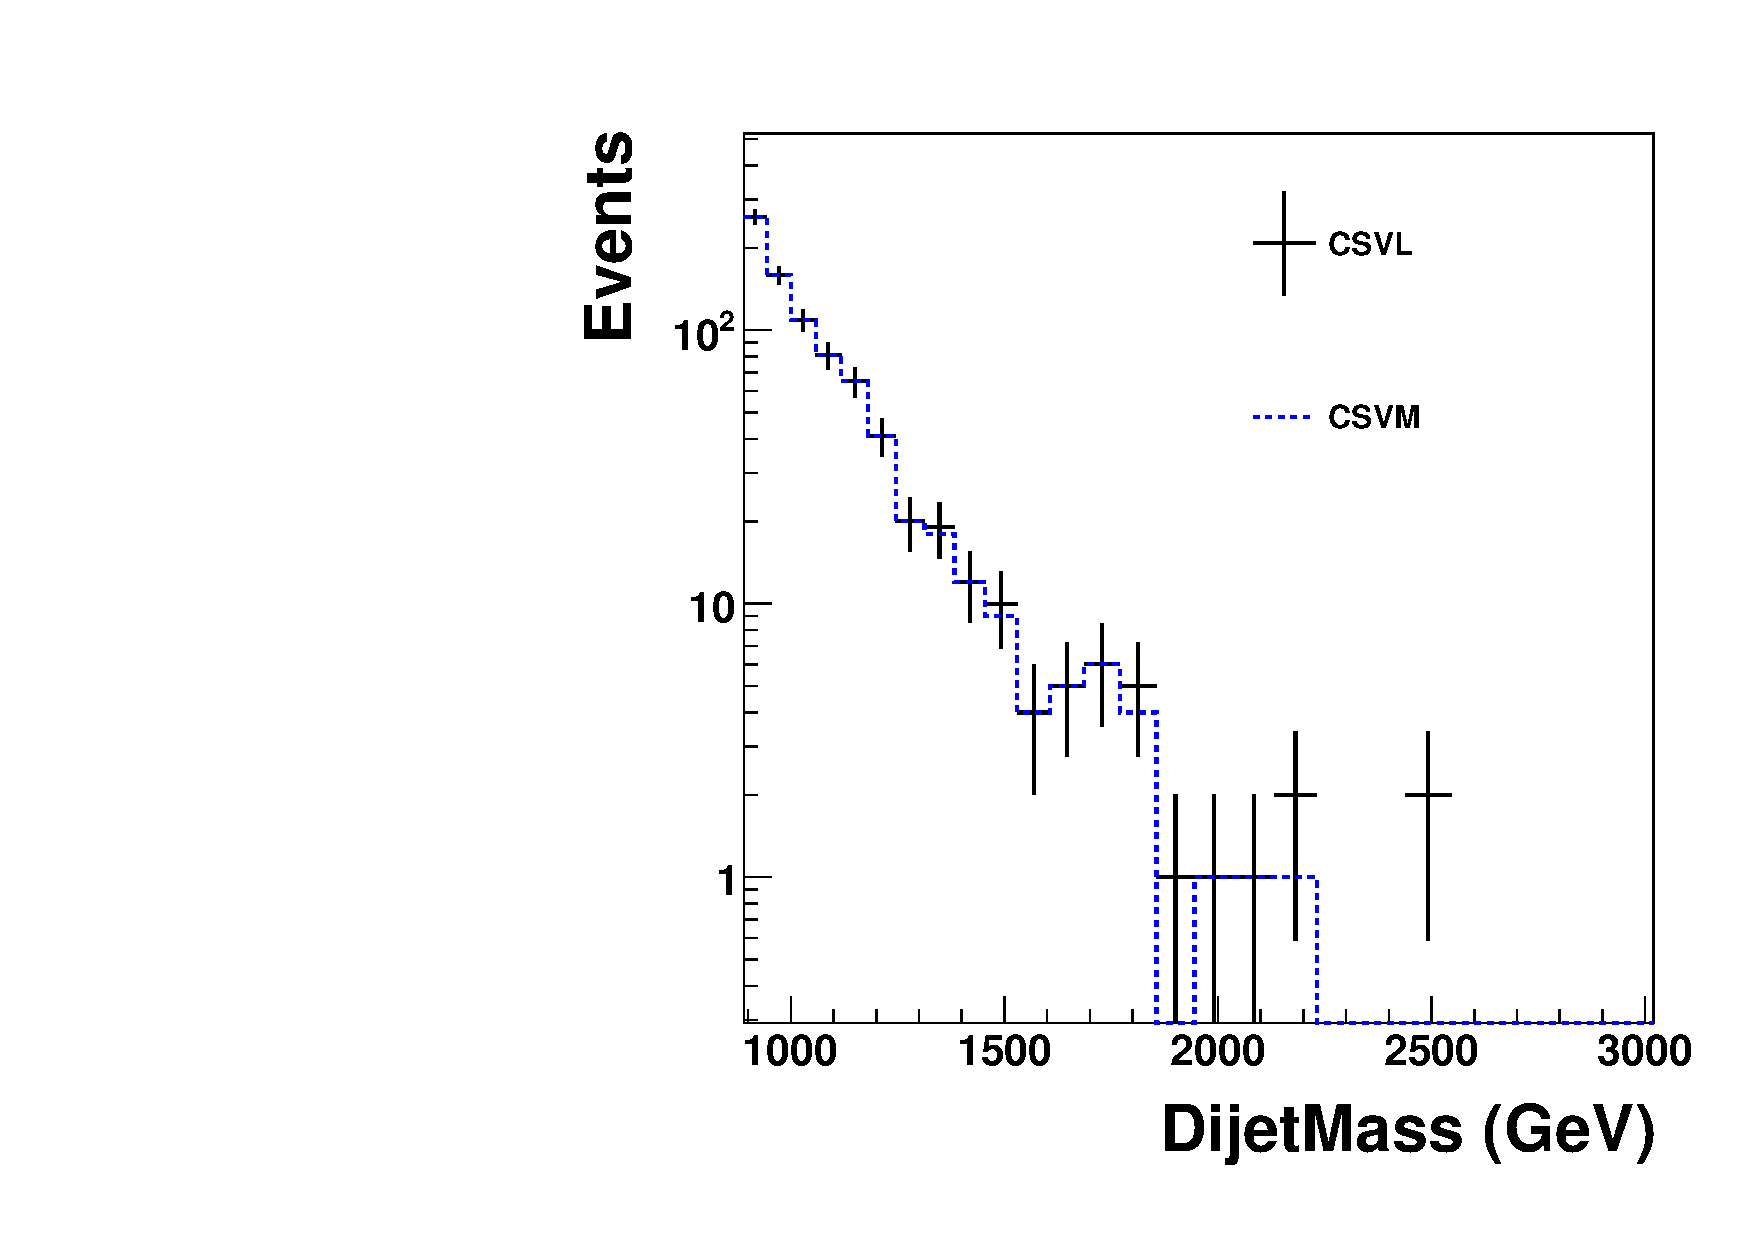
\includegraphics[width=0.7\textwidth]{HbbZqqfigs/CSVMLimits/DijetMass.pdf}
\end{center}
\caption{
DijetMass distribution for using CSVL Vs. CSVM. 
}
\label{fig:HbbCSVMDijetMass}
\end{figure*}

\begin{table}[htbp]
\begin{tabular}{|r|r|r|}
\hline
\multicolumn{1}{|l|}{Resonance(TeV)} & \multicolumn{1}{l|}{CSVM(fb)} & \multicolumn{1}{l|}{CSVL(fb)} \\ \hline
1 & 29.9 & 29.4 \\ \hline
1.5 & 6.86 & 6.98 \\ \hline
2 & 2.98 & 2.67 \\ \hline
\end{tabular}
\caption{Limits on different resonance mass for CSVL VS CSVM.}
\label{table:HbbCSVM}
\end{table}


\begin{figure*}[h!tpb]
\begin{center}
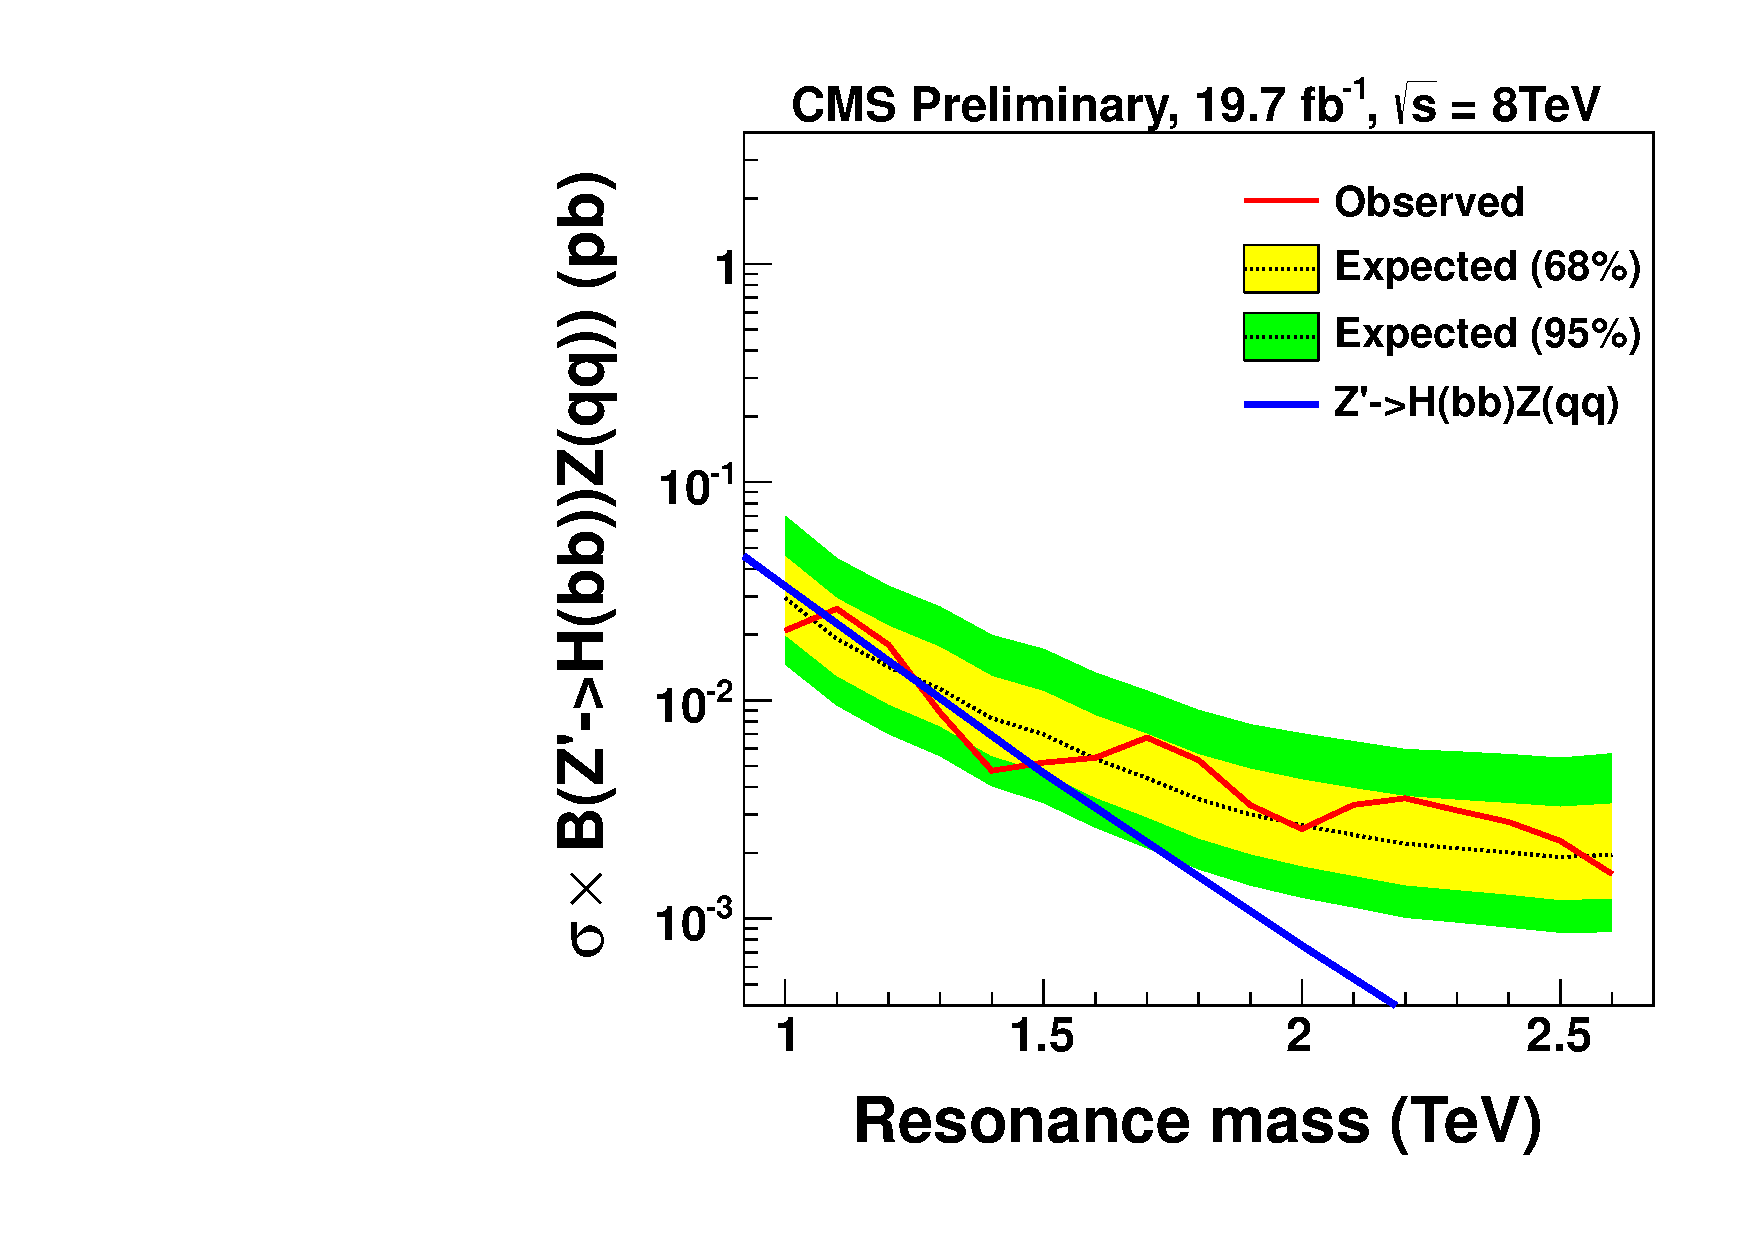
\includegraphics[width=0.49\textwidth]{HbbZqqfigs/Limits/brazilianFlag_Hbb_HbbCombine.pdf}
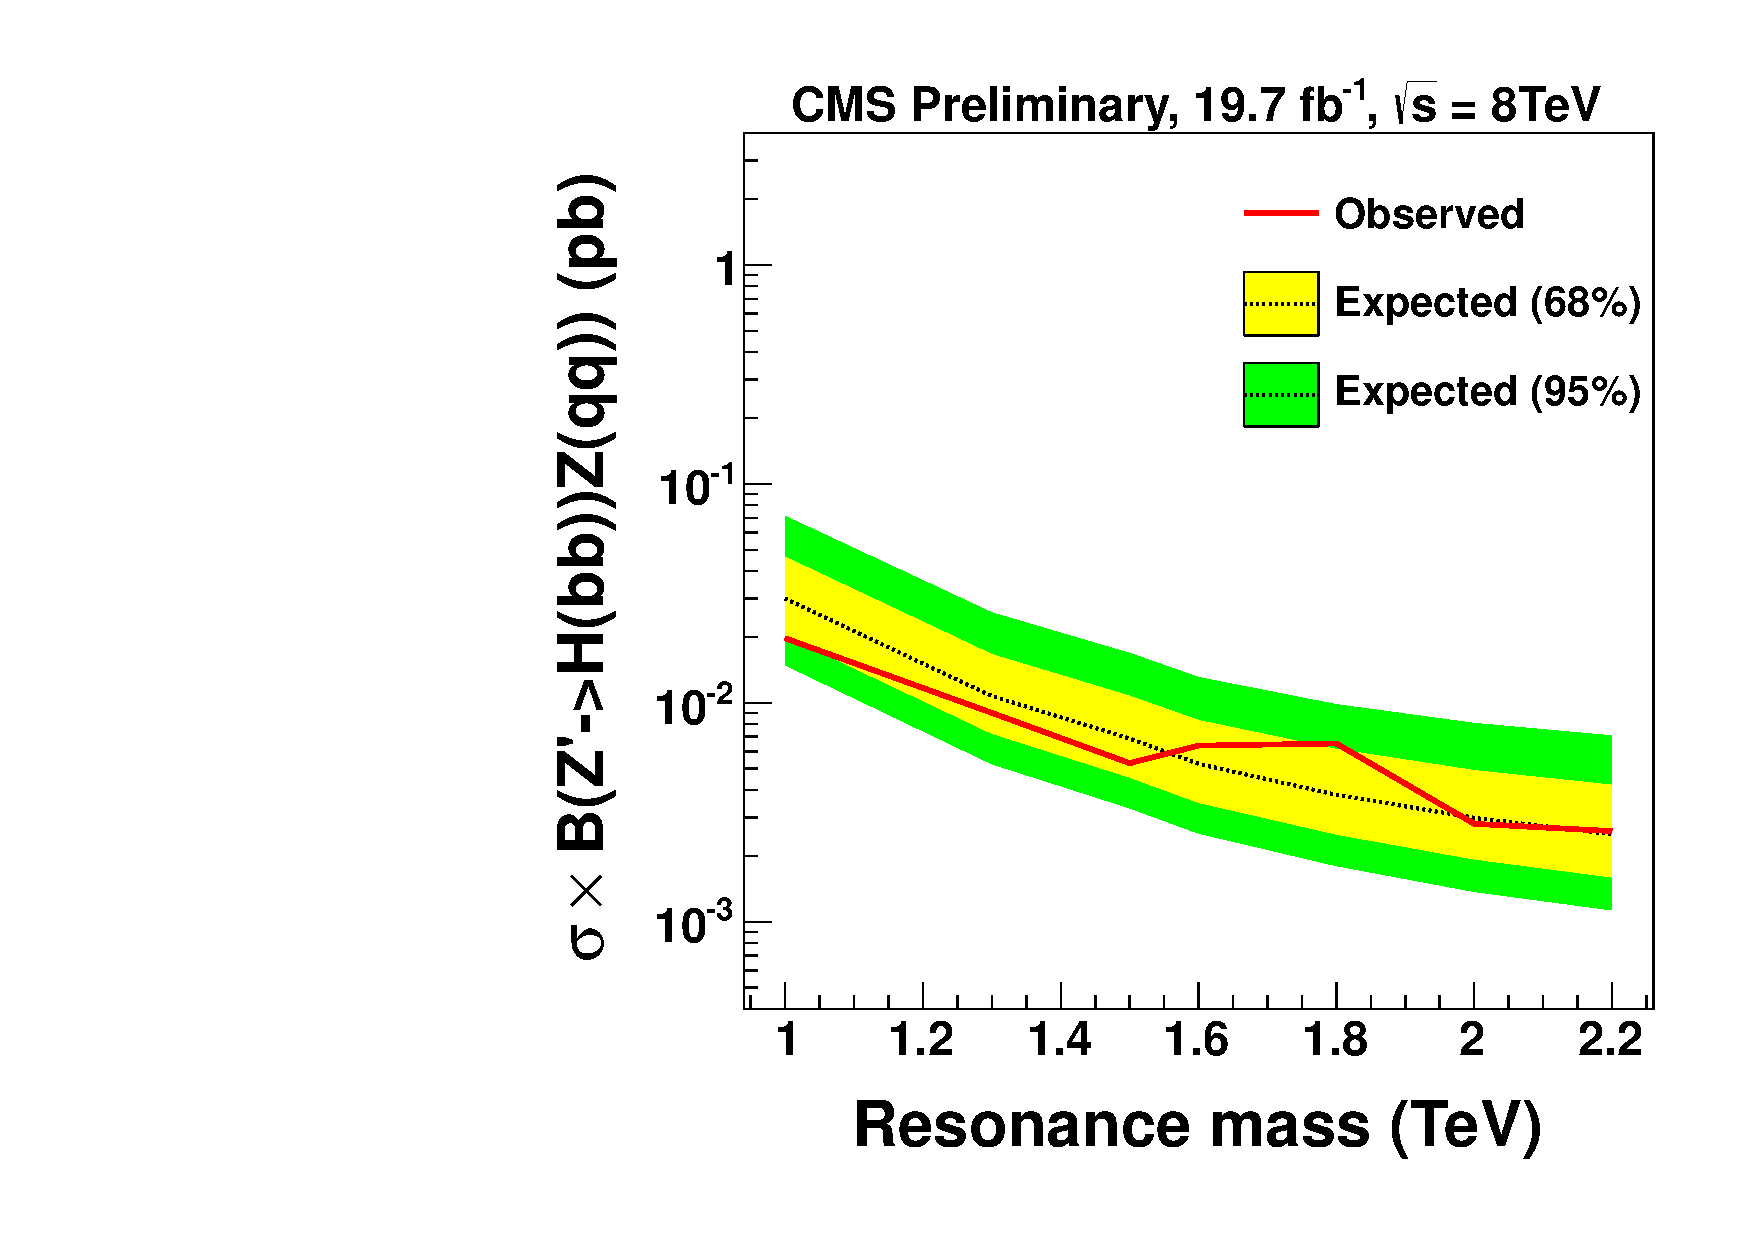
\includegraphics[width=0.49\textwidth]{HbbZqqfigs/CSVMLimits/brazilianFlag_WZ_high_purityHbbCombineCSVM.pdf}
%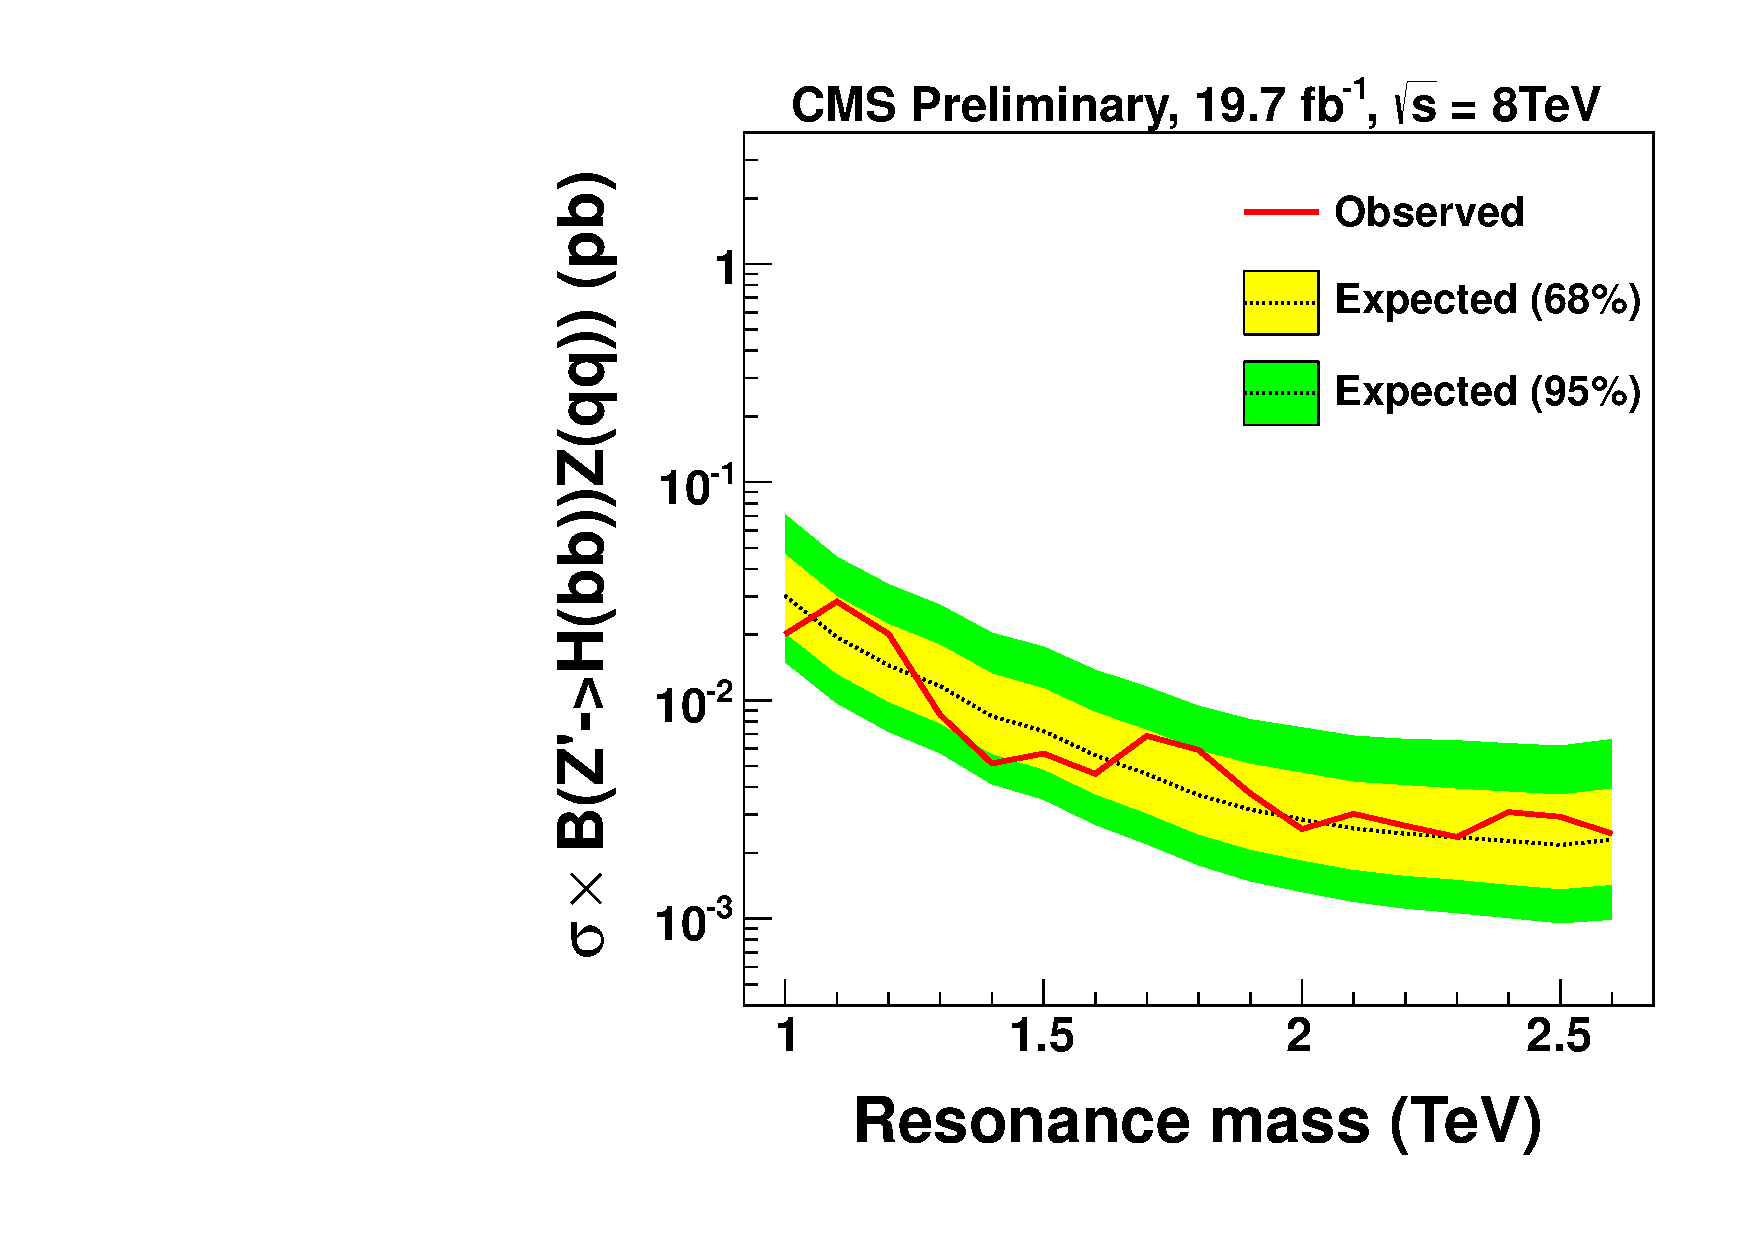
\includegraphics[width=0.49\textwidth]{HbbZqqfigs/Limits/brazilianFlag_Hbb_HbbHighP.pdf}
%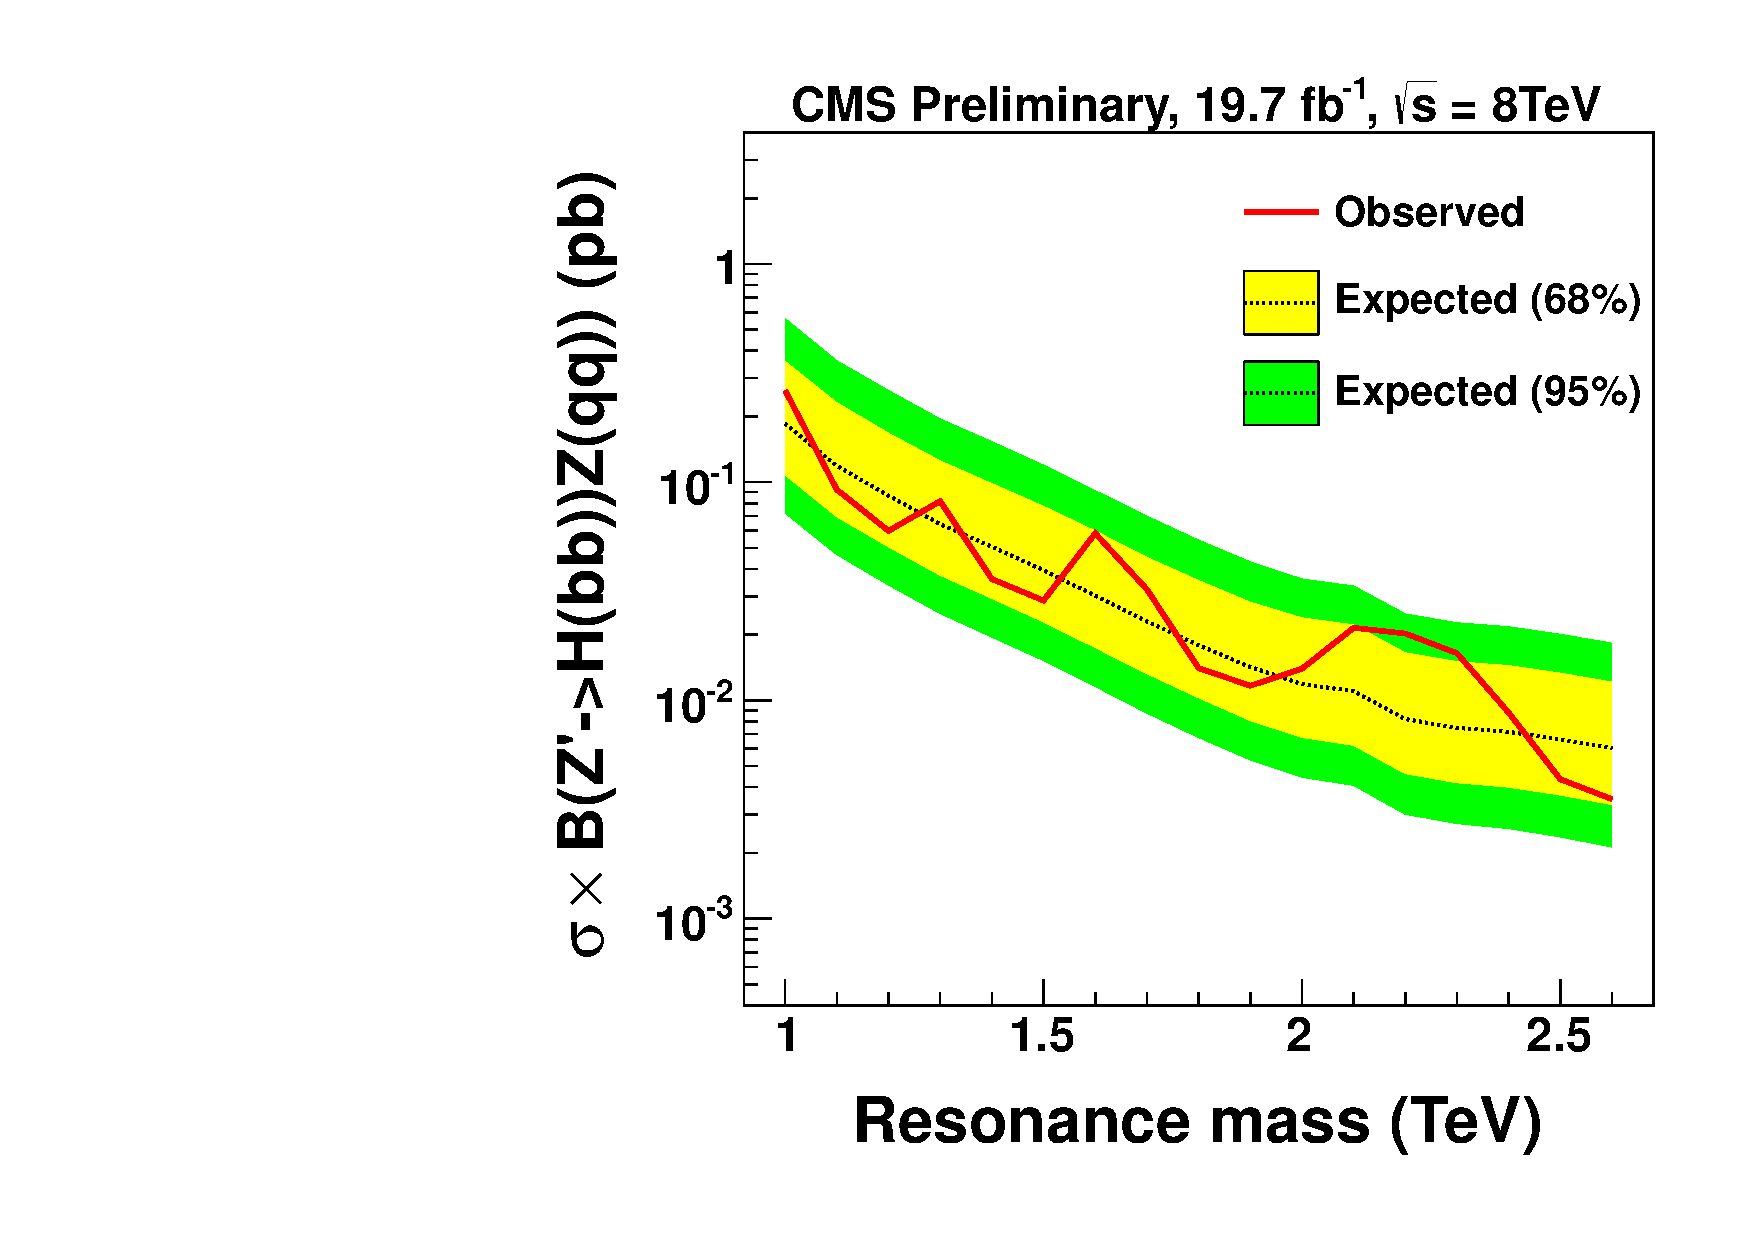
\includegraphics[width=0.49\textwidth]{HbbZqqfigs/Limits/brazilianFlag_Hbb_HbbLowP.pdf}
\end{center}
\caption{
Comparison for limits using CSVL fat jet b tagging(left), and CSVM fat jet b tagging(right). 
%Expected and observed limits for H(bb)Z(qq) search. The combined limit is on top. 
%The high purity is on the bottom left. the low purity V-tagging on bottom right.   
%  The predicted cross sections as a function of resonance mass for the considered benchmark models are overlaid.
}
\label{fig:HbbLimitsCompare}
\end{figure*}


\clearpage
